\subsection{Estado de fuente y usos}

Para identificar los movimientos que ocurren en el balance general entre periodos es necesario identificar el estado. Según \textcite{gerencie_2020} " \textit{El estado de fuentes y usos, que básicamente es lo que se hace con el estado de cambios en la situación financiera, se de termina a partir del balance general, de tal manera que se calculan las variaciones (aumentos y disminuciones) de los activos, pasivos y el patrimonio del periodo actual frente a un periodo anterior}" .

\vspace{2mm}
\begin{minipage}{0.9\textwidth}
\centering
\captionof{table}[{Estado de fuente y usos
}]{ Estado de fuente y usos. }
\label{financiacion}
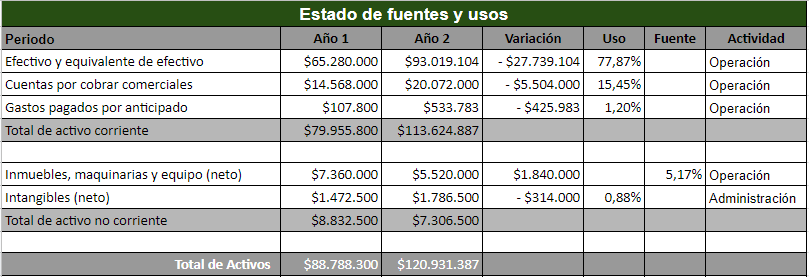
\includegraphics[width=0.8\textwidth]{Images/estadoUsos1.png}
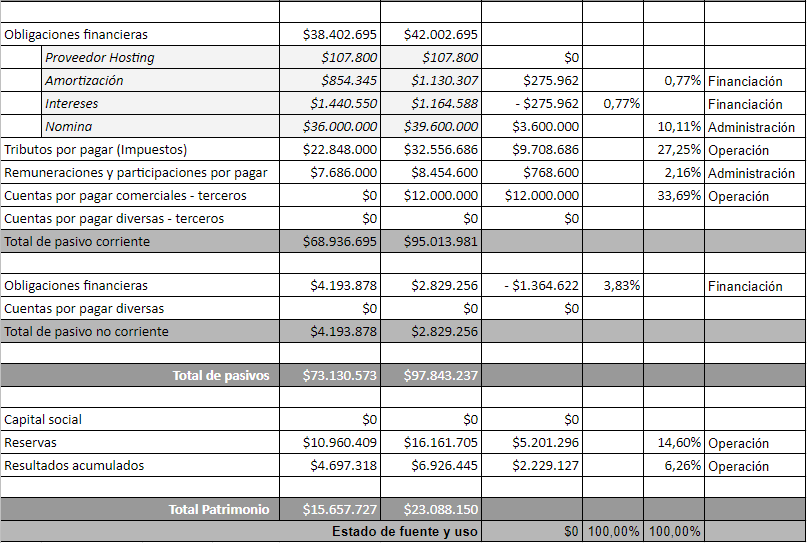
\includegraphics[width=0.8\textwidth]{Images/estadoUsos2.png}
\fnote{Nota. \textup{Fuente : Autores}}
\end{minipage}

En el siguiente resumen de la tabla \ref{resumen} se evidencian todas las fuentes y usos que tiene la empresa. Se observa una cantidad mayor de ingresos que de egresos.

\vspace{2mm}
\begin{minipage}{0.9\textwidth}
\centering
\captionof{table}[{Resumen fuente y usos}]{ Resumen fuente y usos. }
\label{resumen}
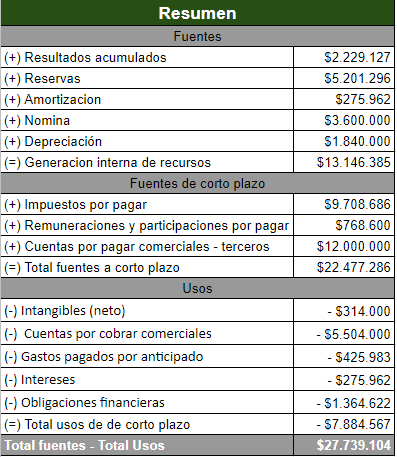
\includegraphics[\textwidth]{Images/resumen.png}
\fnote{Nota. \textup{Fuente : Autores}}
\end{minipage}
